\documentclass[20pt, twoside]{extbook}
\usepackage[utf8]{inputenc}
\usepackage{graphicx}
\usepackage{multicol}
\usepackage{marginnote}
\usepackage{etoolbox}
\usepackage{setspace}
\usepackage[font={small,it}]{caption}
\usepackage{titlesec}
\usepackage{subfig}
\usepackage{float}
%\usepackage[chapter]{placeins}
\usepackage[latin.classical]{babel}

\captionsetup[figure]{labelfont={bf},labelformat={default},labelsep=none,name={},belowskip=-10pt}


\titleformat{\chapter}
{\normalfont\bfseries}
{}{0em}{}
\titlespacing*{\chapter}{0pt}{-50pt}{20pt}

\renewcommand{\thefigure}{}

\let\oldmarginpar\marginpar
\renewcommand\marginpar[1]{\-\oldmarginpar[\raggedleft\scriptsize #1]%
{\raggedright\scriptsize #1}}

\usepackage[top=1.5cm, bottom=2cm, outer=7cm, inner=2cm, heightrounded, marginparwidth=6.25cm, marginparsep=0.5cm]{geometry}
\marginparpush 0.5ex
\setlength{\columnsep}{1cm}
\newcommand{\rnc}[1]
    {\MakeUppercase{\romannumeral #1}}
\parskip 1.5ex
\pagestyle{plain}
\begin{document}

\chapter{CAPITULUM PRIMUM}

\begin{figure}[p]
    \hspace*{-2.5cm}
    \makebox[\linewidth]{
        \setlength{\fboxsep}{0pt}
        \fbox{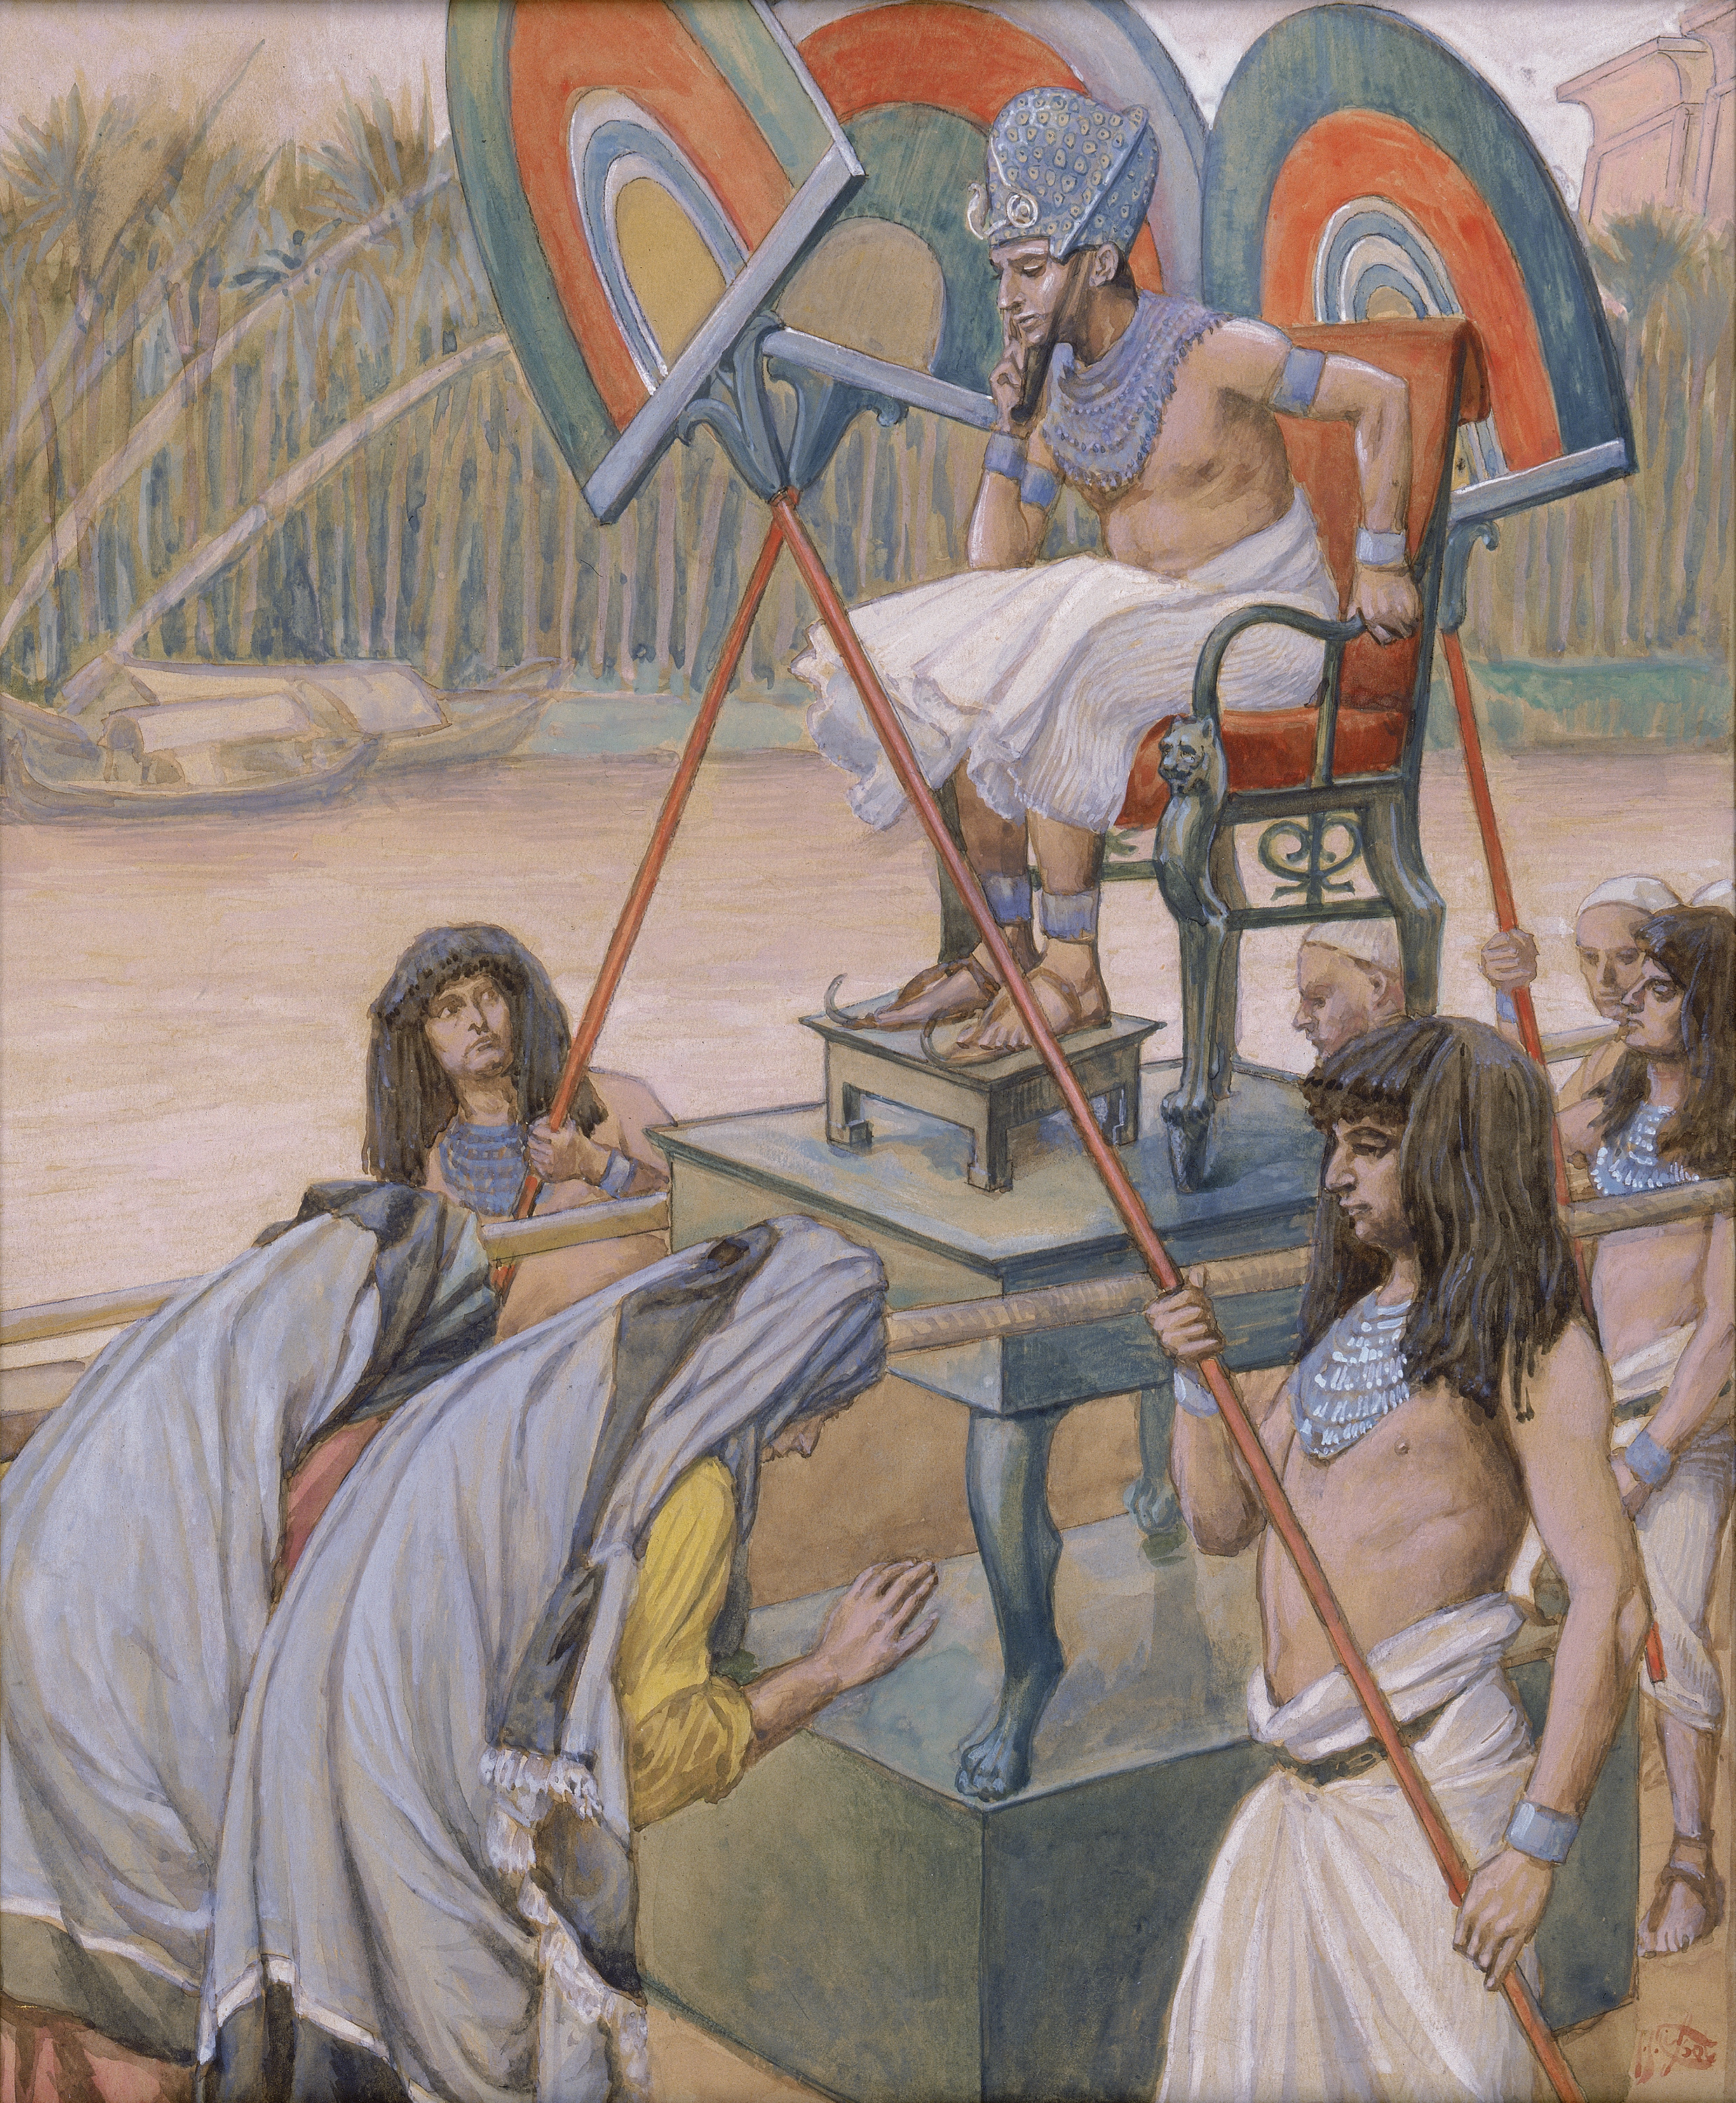
\includegraphics[width=1.3\linewidth]{midwives}}
    }
    \caption{\hspace*{-4.5cm}Obstetricēs et Rēx}
\end{figure}

\marginpar{quasi: velut}[In Aegyptō] fīliī Isrāēl crēvērunt, et quasi\marginpar{germināre: emmitere germina (ea quae ex plantīs veniunt: semen, fructus, cēt.)} germinantēs multiplicātī sunt:
ac rōborātī \marginpar{rōborāre: firmāre; virēs addere}nimis, implēvērunt terram.

Surrēxit intereā rēx novus super Ægyptum, quī ignōrābat Ioseph.
Et ait ad populum suum: ``Ecce, populus fīliōrum Isrāēl multus, et fortior nōbīs est.
\marginpar{ingruere: cum vi accedere}Venīte, sapienter opprimāmus eum, nē forte multiplicētur: et sī ingruerit contrā nōs bellum, addātur inimīcīs nostrīs, expugnātisque nōbīs ēgredi\-ātur dē terrā.''\marginpar{\begin{center}
\includegraphics{tab}\\tabernaculum, -ī (n)\end{center}tabernaculum quoque significat aedificium sacrum, ad formam tabernaculī}

\marginpar{praeposuit eīs magistrōs operum: dedit magistrīs potestatem super opera fīliōrum Isrāēl}
Præposuit itaque eīs magistrōs operum, ut aff-līgerent eōs oneribus: 
ædificaveruntquē urbēs tabernāculōrum Pharaōnī, Phithom et Ramessēs.
Quantōque opprimēbant eōs, tantō magis multiplicābantur, et crēscē\-bant: 
ōderantque fīliōs Isrāēl Ægyptiī, et afflīgēbant \marginpar{illūdere: deridēre}illūdentēs eīs,
atque ad amāri\-tūdinem perdūcēbant vītam eōrum operibus dūrīs \marginpar{lutum, -ī(n): terra humida}lutī et lateris, omnīque famulātū, quō in terræ operibus premēbantur. 
Dīxit autem rēx Ægyptī \marginpar{obstetrix, -īcis(f): femina quae iuvat feminam gravidam parere} obstetrīcibus Hebræōrum, quārum ūna vocā\-bātur Sephora, altera Phu\-a, 
præcipiēns eīs: ``Quandō obstetrīcābitis Hebræās, et \marginpar{partus, -ūs (m): actus pariendi} partus tempus advēnerit: sī masculus fuerit, interficite eum: sī fēmina, \marginpar{reservāre: servāre, conservāre}reservātē.''

\marginpar{nōn fēcērunt iuxtā praeceptum regis: non parent praeceptō rēgis}\marginpar{mas, maris(m): homo (vel animal) masculinus}Timuērunt autem obstetrīcēs Deum, et nōn fēcērunt iuxtā præceptum rēgis Ægyptī, sed cōnservābant marēs. 
Quibus ad sē accersītis, rēx ait: ``Quidnam est hoc quod facere voluistis, ut puerōs servārētis?''

Quæ respondērunt: ``Nōn sunt Hebreæ sīcut Ægyptiæ mulierēs: ipsæ enim obstetrīcandī habent scientiam, et priusquam veniāmus ad eās, pariunt.''

\marginpar{cōnfortāre: fortem facere, consolārī}Bene ergō fēcit Deus obstetrīcibus: et crēvit populus, cōnfortātusque est nimis.
Et quia timuērunt obstetrīcēs Deum, ædificāvit eīs domōs.
Præcēpit ergō Pharaō omnī populō suō, dīcēns: ``Quidquid masculīnī sexūs nātum fuerit, in flūmen prōiicite: quidquid fēminīnī, reservātē.''
\begin{figure}[bp]
    \hspace*{-2.5cm}
    \makebox[\linewidth]{
        \setlength{\fboxsep}{0pt}
        \fbox{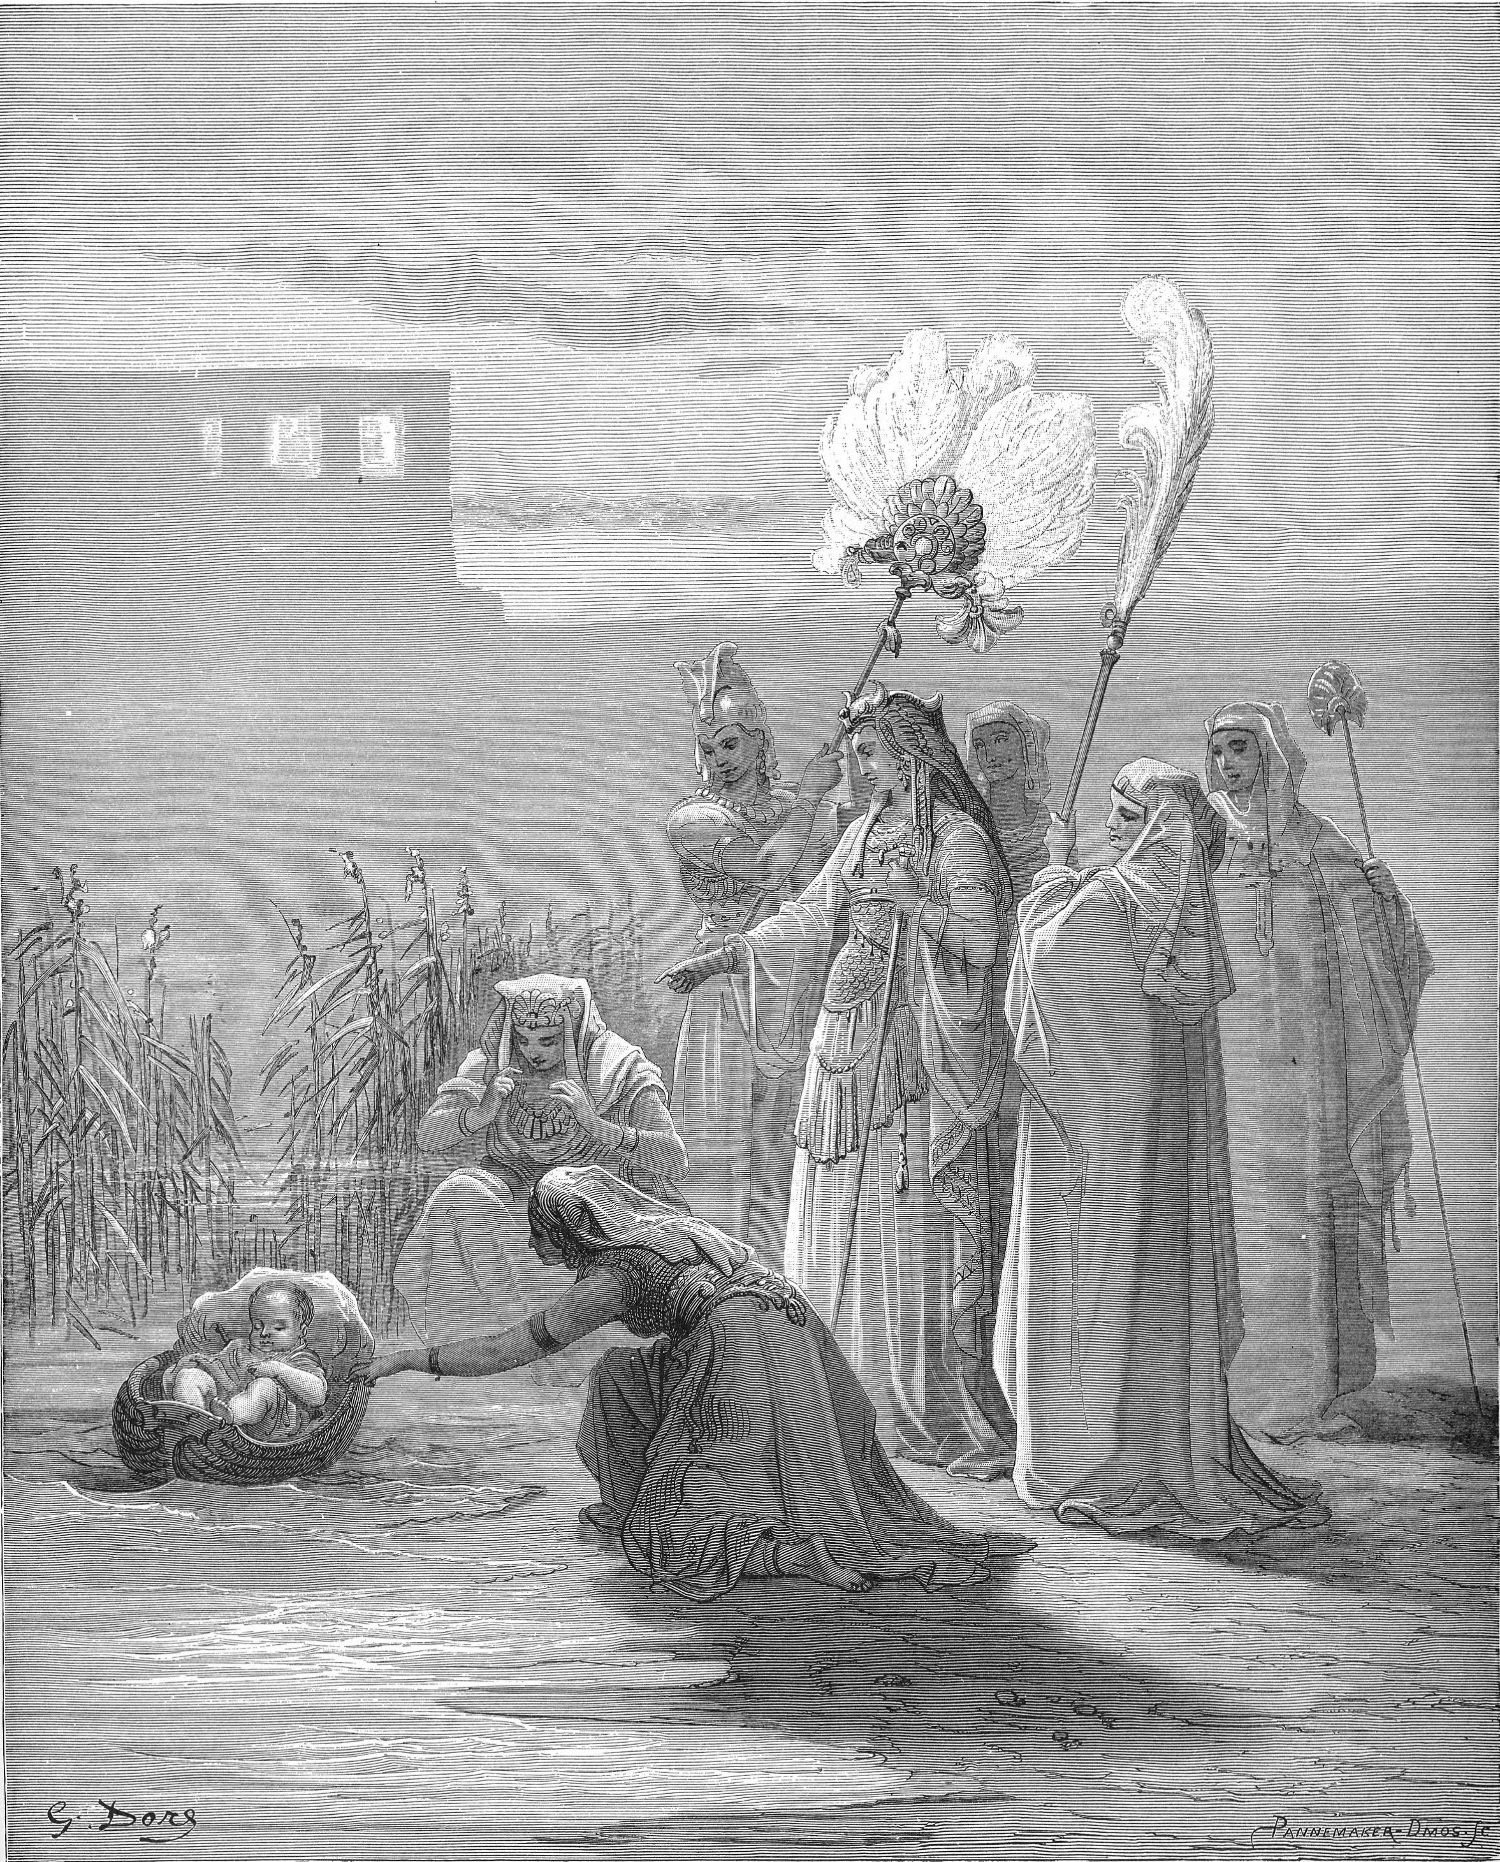
\includegraphics[width=1.3\linewidth]{babymoses.jpg}}
    }
    \caption{\hspace*{-4cm}Infans Moysēs}
\end{figure}

\chapter{CAPITULUM SECUNDUM}
\marginpar{stirps, stirpis(m/f): stricto sensu est truncus arboris, ergo etiam origo est generis in familiis}Ēgressus est post hæc vir dē domō Levī: et accēpit uxōrem stirpis suæ.
Quæ concēpit, et peperit fīlium : et vidēns eum ēlegantem, abscondit tribus mēnsibus.
\marginpar{scirpeus/a/um: ex scirpīs factus}
\marginpar{linere: rem aliquam liquidam aut mollem alteri superinducere}
\marginpar{bitūmen, -inis(n): limus pinguis et sulphureus ē terrā emergens pluribus locīs}
\marginpar{pix, picis (f): rēs ātra quae fit ex liquōre crassō arborum coctō}
\marginpar{cārex, cāricis (f):  herba acuta et durissima, sparto similis}
\marginpar{cārectum, -ī (n): locus caricibus plenus}

\begin{figure}[hp]
    \begin{minipage}[hbp]{0.5\linewidth}
        \centering
        
\includegraphics{fisc}
        \caption{fiscella, -ae(f)}
    \end{minipage}%
    \begin{minipage}[hbp]{0.5\linewidth}
        \centering
        
\includegraphics{brush}
        \caption{scirpus, -ī(m)}
    \end{minipage}
\end{figure}

Cumque iam cēlāre nōn posset, sūmpsit fiscellam scirpeam,
et līnīvit eam bitūmine ac pice:
posuitque intus īnfantu\-lum, et exposuit eum in cārectō rīpæ flū\-minis,
stante procul sorōre eius, et cōnsī\-derante ēventum reī.
Ecce autem dēscendē\-bat fīlia Pharaōnis ut lavārē\-tur in flūmine.\marginpar{crepīdo, -inis (f): litus maris vel ripa fluminis, quae saxis, aut lapideo margine plerumque sternebantur}\marginpar{alveus, -ī (m): fossa, per quam fluvius defluit} Et puellæ eius gradiēbantur per crepīdinem alveī.
\marginpar{papyrio, -ōnis (m): locus papyrīs consitus}
Quæ cum vīdisset fiscellam in papȳ\-riōne,
mīsit ūnam ē famulābus suīs: et al\-lātam aperiēns,
cer\-nēnsque in eā parvulum vāgientem,
miserta eius, ait: ``Dē īnfantibus Hebræōrum est hīc.''

Cui soror puerī: ``Vīs,'' inquit, ``ut vā\-dam, et vōcem tibi mulierem hebræam,
quæ nūtr\-īre possit īnfantulum?''

Respondit: ``Vāde.''

Perrēxit puella et vocāvit mātrem suam.
Ad quam locūta fīlia Pharaōnis: ``Accipe,'' ait, ``puerum istum, et nūtrī mihi: ego dabō tibi mercēdem tuam.''

Suscēpit mulier, et nūtrīvit puerum: adultumque trādidit fīliæ Pharaōnis. 
Quem illa adoptāvit in locum fīliī,
vocāvitque nōmen eius Moysēs, dīcēns: ``Quia dē aquā tulī eum.''

In diēbus illīs postquam crēverat Moysēs, ēgressus est ad frātrēs suōs:
\marginpar{percutere: pulsare, afficere, et quasi vulnerare dolore}vīditque afflīctiōnem eōrum, et virum ægyptium percutientem quemdam dē Hebræīs frātribus suīs.
Cumque circumspexisset hūc atque illūc,
et nūllum adesse vīdisset,
\marginpar{abscondere: rem aliquam aliquo in loco ponere, ut celetur}
\marginpar{sabulum, -ī: arena}percussum Ægyptium abscondit sabulō.
\marginpar{rixāre: contendere}Et ēgressus diē alterō cōnspexit duōs Hebræōs rixantēs:
dīxitque eī quī faciēbat iniūriam: ``Quārē percutis proximum tuum?''

Quī respondit: ``Quis tē cōnstituit prīn\-cipem et iūdicem super nōs?
num occīdere mē tū vīs, sīcut heri occīdistī Ægyptium?''

Timuit Moysēs, et ait: ``Quōmodo palam factum est verbum istud?''

Audīvitque Pharaō sermōnem hunc, et quærēbat occīdere Moysēn:
quī fugiēns dē cōnspectū eius, morātus est in terrā Madiān,
\marginpar{puteus, -ī (m): aedificium (et foramen) ex quo aqua excipitur}et sēdit iuxtā puteum.
Erant autem sacerdōtī Madian septem fīliæ,
quæ vēnērunt ad hauriendam aquam:
\marginpar{adaquāre: aquam dāre}et implētīs canālibus adaquāre cupiēbant gregēs patris suī.
Supervēnēre pāstōrēs, et ēiēcērunt eās:
surrēxit\-que Moysēs, et dēfēnsīs puellīs, adaquāvit ovēs eārum. 
Quæ cum revertissent ad Raguel patrem suum, dīxit ad eās:
\marginpar{vēlox, -ōcis: celer}``Cūr vēlō\-cius vēnistis solitō?''

Respondērunt: ``Vir ægyptius līberāvit nōs dē manū pāstōrum:
\marginpar{īnsuper: praeterea}īnsu\-per et hausit aquam nōbīscum, pōtumque dedit ovibus.''

At ille: ``Ubi est?'' inquit: ``quārē dīmī\-sistis hominem? vocātē eum ut comedat pānem.''

Iūrāvit ergō Moysēs quod habitāret cum eō.
Accēpitque Sephoram fīliam eius uxōrem:
quæ peperit eī fīlium, quem vocāvit Gersam, dīcēns:
``Advena fuī in terrā aliēnā.''

Alterum vērō peperit, quem vocāvit Eliezer, dīcēns:
``Deus enim patris meī adiūtor meus ēripuit mē dē manū Pharaōnis.''

Post multum vērō tempore mortuus est rēx Ægyptī:
\marginpar{ingemīscere: dolere; prae animi angustia in sonum prorumpere et queri, suspirare}et ingemīscentēs fī\-liī Isrā\-ēl
propter opera vōciferātī sunt:
\marginpar{vōciferātus/a/um $<$ vōciferārī: vehementer exclamāre}
ascenditque clā\-mor eōrum ad Deum ab operibus.
Et audīvit gemitum eōrum,
\marginpar{pangō, pangere, pepigisse, pactum: constituere, definite statuere}ac recordātus est fœderis quod pepigit cum Abraham, Isaac et Iācōb.
Et respexit Dominus fīliōs Isrāēl et cognōvit eōs.

\chapter{CAPITULUM TERTIUM}

\begin{figure}[h]
    \hspace*{0.5cm}
    \setlength{\fboxsep}{0pt}
    \fbox{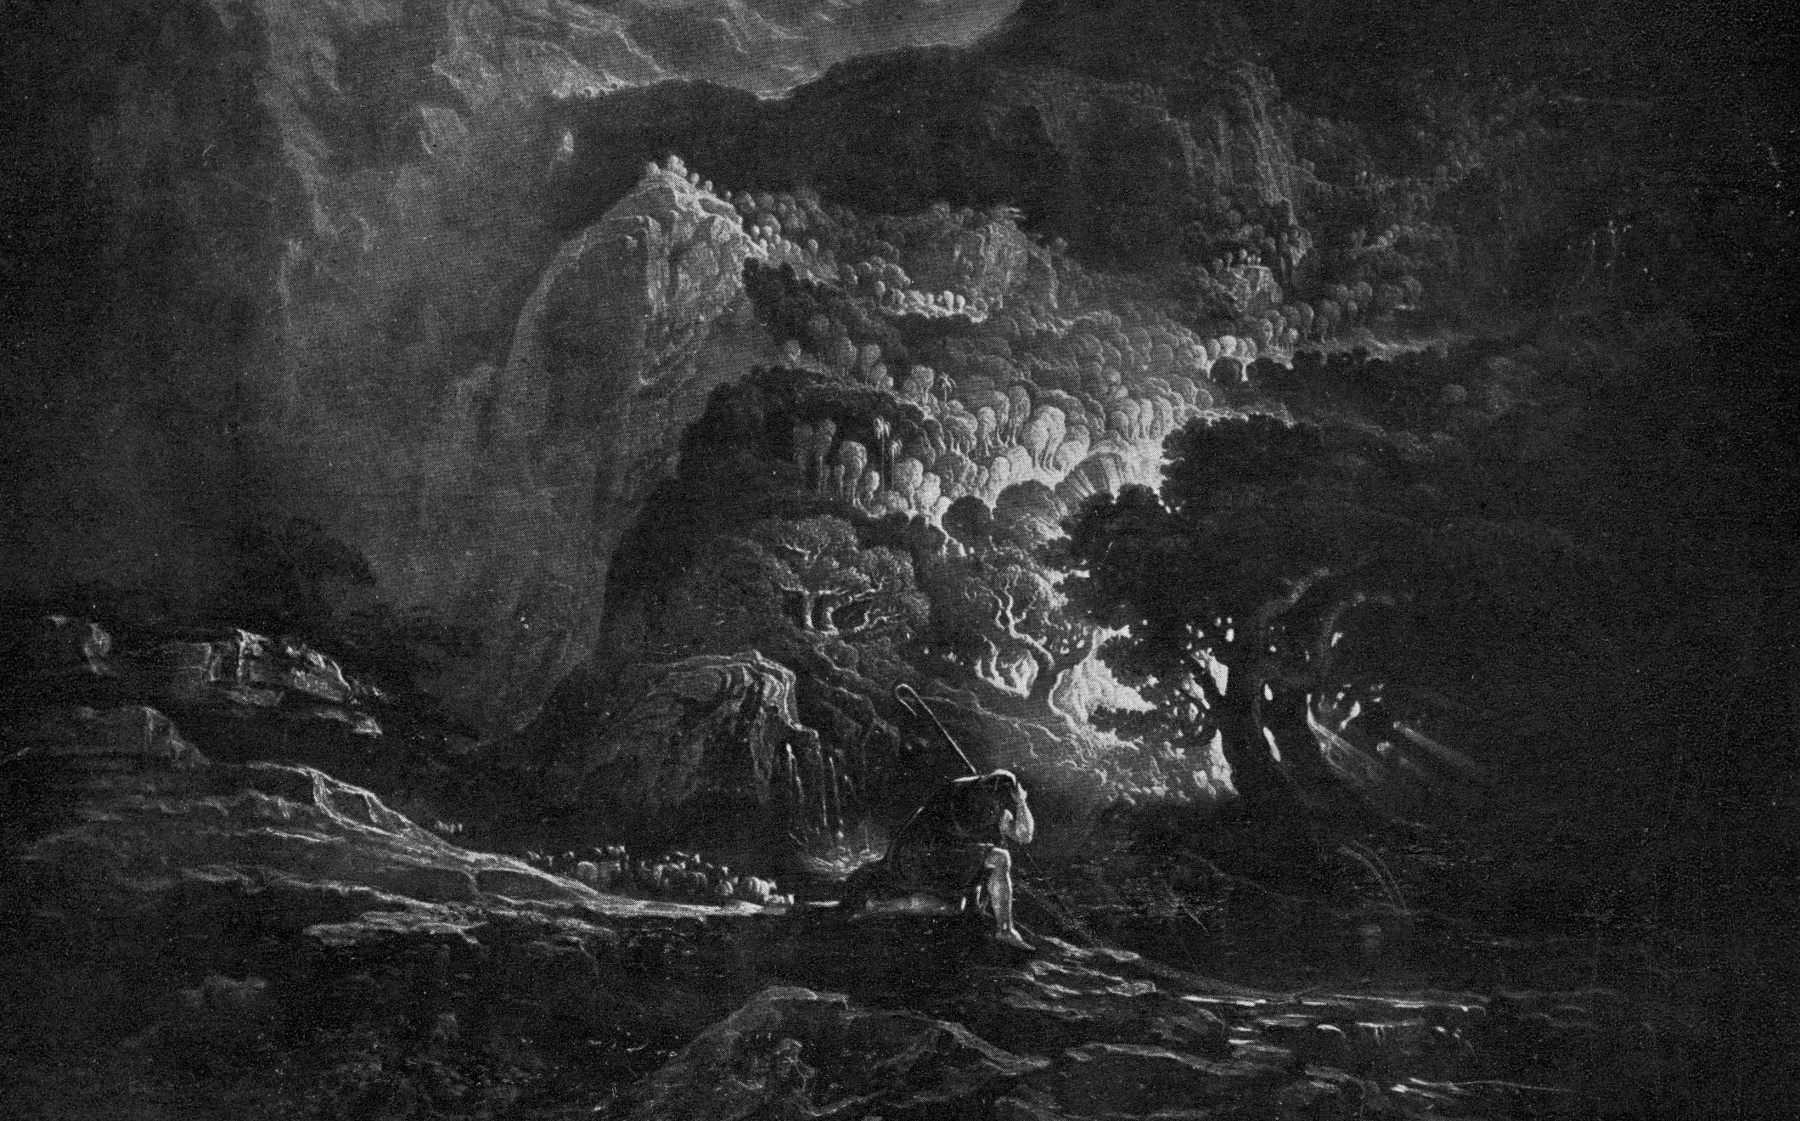
\includegraphics[width=1.3\linewidth]{burning_bush.jpg}}
    \caption{\hspace*{4cm}Rubus Ardēns}
\end{figure}

Moysēs autem pāscēbat ovēs Iethrō socerī suī sacerdōtis Madian:
\marginpar{mināre: cōgere animālia}cumque mināsset gregem ad interiōra dēsertī,
venit ad montem Deī Horeb.
\marginpar{rubus, -ī (m): quaedam planta spinosa}
Appāruitque eī Dominus in flammā ignis dē mediō rubī:
\marginpar{ārdēre: igne flagrāre}\marginpar{combūrere: igne cōnsūmere}et vidēbat quod rubus ārdēret, et nōn combūrerētur.
Dīxit ergō Moysēs : ``Vādam, et vidēbō vīsi\-ōnem hanc magnam, quārē nōn combūrātur rubus.''

Cernēns autem Dominus quod pergeret ad videndum,
vocāvit eum dē mediō rubī, et ait: ``Moysēs, Moysēs.''

Quī respondit: ``Adsum.''

\marginpar{calceāmentum, -ī: quod pedī induitur}At ille: ``Nē appropiēs,'' inquit, ``hūc: solve calceāmentum dē pedibus tuīs: locus enim,
in quō stās, terra sāncta est.'' 

Et ait: ``Ego sum Deus patris tuī, Deus Abraham, Deus Isaac et Deus Iācōb.''

Abscondit Moysēs faciem suam: nōn enim audēbat aspicere contrā Deum.

\marginpar{afflīctiō, -ōnis (f): rēs quae valde displicet, vexat, nocet}Cui ait Dominus: ``Vīdī afflīctiōnem populī meī in Ægyptō,
\marginpar{{\bf duritia, -ae (f)} $<$ durus/a/um}et clāmōrem eius audīvī propter dūritiam eōrum quī præsunt operibus:
et sciēns dolōrem eius, dēscendī ut libērem eum dē manibus Ægyptiōrum,
\marginpar{spatiōsus/a/um: multum spatiī habēns}et ēdūcam dē terrā illā in terram bonam, et spatiōsam,
\marginpar{lac, lactis (n): quod infantēs bibunt}in terram quæ fluit lacte et melle,
ad loca Chananæī et Hethæī, et Amorrhæī, et Pherezæī, et Hevæī, et Iebusæī.
Clāmor ergō fīliōrum Isrāēl venit ad mē: vīdīque afflīctiōnem eōrum,
qua ab Ægyptiīs opprimuntur.
Sed vēnī, et mittam tē ad Pharaōnem,
ut ēducās populum meum, fīliōs Isrāēl, dē Ægyptō.''

Dīxitque Moysēs ad Deum: ``Quis sum ego ut vādam ad Pharaōnem,
et ēdūcam fīliōs Isrāēl dē Ægyptō?''

Quī dīxit eī: ``Ego erō tēcum: et hoc habēbis signum,
quod mīserim tē: cum ēdūx\-erīs populum meum dē Ægyptō,
immolābis Deō super montem istum.''

Ait Moysēs ad Deum: ``Ecce ego vādam ad fīliōs Isrāēl,
et dīcam eīs: Deus patrum vestrōrum mīsit mē ad vōs.
Sī dīxerint mihi: `Quod est nōmen eius?' quid dīcam eīs?''

Dīxit Deus ad Moysēn: ``EGO SUM QUĪ SUM.'' Ait: ``Sīc dīcēs fīliīs Isrāēl: `QUĪ EST mīsit mē ad vōs.' ''

Dīxitque iterum Deus ad Moysēn: ``Hæc dīcēs fīliīs Isrāēl:
Dominus Deus patrum vestrōrum, Deus Abraham, Deus Isaac et Deus Iācōb,
\marginpar{in æternum: semper} mīsit mē ad vōs: hoc nōmen mihi est in æternum,
\marginpar{memoriāle, -is (n): id quod memorandum est}et hoc memoriāle meum in generātiōnem et generātiōnem.''

``Vāde, et congregā seniōrēs Isrāēl,
et dīcēs ad eōs: Dominus Deus patrum vestrōrum appāruit mihi,
Deus Abraham, Deus Isaac et Deus Iācōb,
\marginpar{vīsitāns vīsītāvī: vīsitāvī (rhētoricē paene idem iterum dicit)}dīcēns: Vīsitāns vīsitāvī vōs: et vīdī omnia quæ accidērunt vōbīs in Ægyptō.
Et dīxī ut ēdūcam vōs dē afflīctiōne Ægyptī in terram Chananæī,
et Hethæī, et Amorrhæī, et Pherezæī, et Hevæī, et Iebusæī,
ad terram fluentem lacte et melle.''

``Et audient vōcem tuam: ingrediērisque tū,
et seniōrēs Isrāēl, ad rēgem Ægyptī, et dīcēs ad eum:
Dominus Deus Hebræōrum vocāvit nōs:
\marginpar{sōlitūdo, -inis $<$ solus/a/um: regio deserta; locus ubi nemo vel unus habitat}ībimus viam trium diērum in sōlitūdinem,
\marginpar{immolāre: sacrificium facere}ut immolēmus Dominō Deō nostrō.''

``Sed ego sciō quod nōn dīmittet vōs rēx Ægyptī
ut eātis nisi per manum validam.
Extendam enim manum meam, et percutiam Ægyptum
in cūnctīs mīrābilibus meīs, 
quæ factūrus sum in mediō eōrum:
post hæc dīmittet vōs.
Dabōque grātiam populō huic cōram Ægyptiīs:
\marginpar{vacuī: id est, sine rēbus}et cum ēgrediēminī, nōn exībitis vacuī:
\marginpar{vīcīnus/a: qui prope habitat}sed postulābit mulier ā vīcīnā suā
et ab hospitā suā, vāsa argentea et aurea, ac vestēs:
\marginpar{spoliāre: capere rēs aliōrum hominum}pōnētisque eās super fīliōs et fīliās vestrās, et spoliābitis Ægyptum.''

\chapter{CAPITULUM QUARTUM}

\begin{figure}[h]
    \hspace*{0.5cm}
    \setlength{\fboxsep}{0pt}
    \fbox{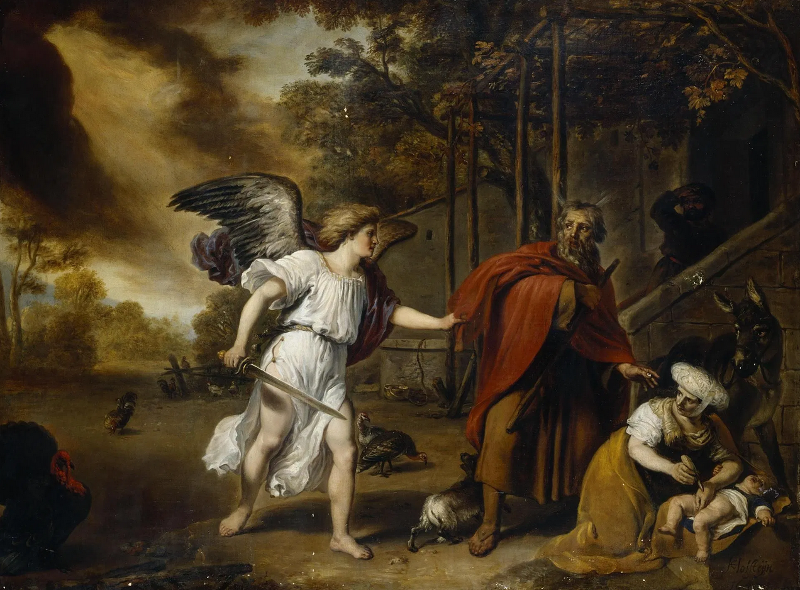
\includegraphics[width=1.3\linewidth]{inn.png}}
    \caption{\hspace*{4cm}Sephora in Deversōriō}
\end{figure}

Respondēns Moysēs ait: ``Nōn crēdent mihi, neque audient vōcem meam, sed dīcent:
Nōn appāruit tibi Dominus.''

Dīxit ergō ad eum: ``Quid est quod tenēs in manū tuā?''

Respondit: ``Virga.''

\marginpar{prōiicere: procul iacere; abiicere} Dīxitque Dominus: ``Prōiice eam in terram.''

\marginpar{coluber, -brī (m): serpens}Prōiēcit, et versa est in colubrum, ita ut fugeret Moysēs. 

Dīxitque Dominus: ``Extende manum tu\-am, et apprehende caudam eius.''

Extendit, et tenuit, versaque est in virgam.
``Ut crēdant,'' inquit, ``quod appāru\-erit tibi Dominus Deus patrum suōrum,
De\-us Abraham, Deus Isaac et Deus Iācōb.''

Dīxitque Dominus rūrsum: ``Mitte manum tuam in sinum tuum.''

\marginpar{{\bf leprōsus/a/um $<$ leprae, -ārum (f)}: morbus qui cutem (exterior pars hominis) deformat}
\marginpar{īnstar + gen: sicut}Quam cum mīsisset in sinum, prōtulit leprōsam īnstar nivis.
``Retrahe,'' ait, ``manum tuam in sinum tuum.''

Retrāxit, et prōtulit iterum,
et erat similis carnī reliquæ.
``Sī nōn crēdiderint,'' inquit, ``tibi, neque audierint
sermōnem signī priōris, crēdent verbō signī sequentis. 
Quod sī nec duōbus quidem hīs signīs crēdiderint,
neque audierint vōcem tuam: sūme aquam flūminis,
\marginpar{āridus/a/um: sine aquā}et effunde eam super āridam, et quidquid hauserīs dē fluviō,
vertētur in sanguinem.''

\marginpar{nūdiustertius: ante duōs diēs}
Ait Moysēs: ``Obsecrō, Domine, nōn sum ēloquēns ab heri et
\marginpar{{\bf ex quō} (tempore)}nūdiustertius: et ex quō locūtus es ad servum tuum,
impedītiōris et tardiōris linguæ sum.''

Dīxit Dominus ad eum: ``Quis fēcit os hominis?
\marginpar{fabricatus/a/um: confectus}
\marginpar{mūtus/a/um: loquī non potest}
\marginpar{surdus/a/um: audīre non potest}
aut quis fabricātus est mūtum et surdum,
\marginpar{caecus/a/um: vidēre non potest}videntem et cæcum? nōnne ego?
Perge, igitur, et ego erō in ōre tuō:
docē\-bōque tē quid loquāris.''

\marginpar{obsecrāre: orāre, precārī}At ille: ``Obsecrō, inquit, Domine,
mitte quem missūrus es.''

Īrātus Dominus in Moysēn, ait: ``Aarōn frāter tuus Lēvītēs,
sciō quod ēloquēns sit: ecce ipse ēgreditur in occursum tuum,
vid\-ēnsque tē lætābitur corde.
Loquere ad eum, et pōne verba mea in ōre eius:
et ego erō in ōre tuō, et in ōre illīus,
et ostendam vōbīs quid agere dēbeātis.
Ipse loquētur prō tē ad populum,
et erit os tuum:
tū autem eris eī in hīs quæ ad Deum pertinent.
Virgam quoque hanc sūme in manū tuā,
in quā factūrus es signa.

\marginpar{socer, socerī (m): pater uxōris}Abiit Moysēs, et reversus est ad Iethrō socerum suum,
dīxitque eī: ``Vādam et revertar ad frātrēs meōs in Ægyptum,
ut videam sī adhūc vīvant.''

Cui ait Iethrō: ``Vāde in pāce.''

Dīxit ergō Dominus ad Moysēn in Madiān: ``Vāde, et revertere in Ægyptum,
mortuī sunt enim omnēs quī quærēbant animam tuam.''

\begin{figure}[hbp]
        \centering
        \setlength{\fboxsep}{0pt}
        \fbox{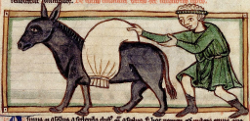
\includegraphics{asinus}}
        \caption{asinus, -ī (m)}
\end{figure}
Tulit ergō Moysēs uxōrem suam, et fīliōs suōs,
et imposuit eōs super asinum: reversusque est in Ægyptum,
portāns virgam Deī in manū suā. Dīxitque eī Dominus revertentī
in Ægyptum: ``Vidē ut omnia ostenta quæ posuī in manū tuā
\marginpar{indūrāre: durum facere}faciās cōram Pharaōne: ego indūrābō cor ejus,
et nōn dīmittet populum. Dīcēsque ad eum: Hæc
\marginpar{prīmōgenitus: natū maior}dīcit Dominus: Fīlius meus prīmōgenitus Isrāēl.
Dīxī tibi: Dīmitte fīlium meum ut serviat mihi;
et nōluistī dīmittere eum:
ecce ego interficiam fīlium tuum prīmōgenitum.''

\marginpar{dīversōrium, -ī (n): aedificium in quō hominēs in itinere possunt dormīre}\marginpar{petra, -ae (f): lapis}Cumque esset in itinere, in dīversōriō
occurrit eī Dominus, et volēbat occīdere eum. 
Tulit idcircō Sephora acūtissimam petram,
\marginpar{praepūtium, -ī (n): illa pars puerī quae circumcīditur}et circumcīdit præpūtium fīliī suī, tetigitque pedēs ejus,
\marginpar{spōnsus/a: quī mox alicui maritus vel uxor erit}et ait: ``Spōnsus sanguinum tū mihi es.''
Et dīmīsit eum postquam dīxerat: ``Spōn\-sus sanguinum ob circumcīsiōnem.''

Dīxit autem Dominus ad Aarōn: ``Vāde in occursum Moȳsī
in dēsertum.'' 

Quī perrēxit obviam eī in montem Deī, et ōsculātus est eum.
Nārrāvitque Moysēs Aarōn omnia verba Dominī quibus miserat eum,
et signa quæ mandāverat. Vēn\-ēruntque simul, et congregāvērunt
cūnctōs seniōrēs fīliōrum Isrāēl.
Locūtusque est Aar\-ōn omnia verba quæ dīxerat Dominus ad Moysēn: et
fēcit signa cōram populō, et crēdidit populus.
Audiēruntque quod vīsit\-āsset Dominus fīliōs Isrāēl,
\marginpar{prōnus/a/um: iacēns in pectore}et respexisset afflīctiōnem illōrum: et prōnī adōrāvērunt.
\end{document}
